%%%%%%%%%%%%%%%%%%%%%%%%%%%%%%%%%%%%%%%%%
% Short Sectioned Assignment
% LaTeX Template
% Version 1.0 (5/5/12)
%
% This template has been downloaded from:
% http://www.LaTeXTemplates.com
%
% Original author:
% Frits Wenneker (http://www.howtotex.com)
%
% License:
% CC BY-NC-SA 3.0 (http://creativecommons.org/licenses/by-nc-sa/3.0/)
%
%%%%%%%%%%%%%%%%%%%%%%%%%%%%%%%%%%%%%%%%%

%----------------------------------------------------------------------------------------
%	PACKAGES AND OTHER DOCUMENT CONFIGURATIONS
%----------------------------------------------------------------------------------------

\documentclass[paper=a4, fontsize=11pt]{scrartcl} % A4 paper and 11pt font size

\usepackage[T1]{fontenc} % Use 8-bit encoding that has 256 glyphs
\usepackage{fourier} % Use the Adobe Utopia font for the document - comment this line to return to the LaTeX default
\usepackage[english]{babel} % English language/hyphenation
\usepackage{amsmath,amsfonts,amsthm} % Math packages
\usepackage{graphicx}

\usepackage{lipsum} % Used for inserting dummy 'Lorem ipsum' text into the template

\usepackage{sectsty} % Allows customizing section commands
\allsectionsfont{\centering \normalfont\scshape} % Make all sections centered, the default font and small caps

\usepackage{fancyhdr} % Custom headers and footers
\pagestyle{fancyplain} % Makes all pages in the document conform to the custom headers and footers
\fancyhead{} % No page header - if you want one, create it in the same way as the footers below
\fancyfoot[L]{} % Empty left footer
\fancyfoot[C]{} % Empty center footer
\fancyfoot[R]{\thepage} % Page numbering for right footer
\renewcommand{\headrulewidth}{0pt} % Remove header underlines
\renewcommand{\footrulewidth}{0pt} % Remove footer underlines
\setlength{\headheight}{13.6pt} % Customize the height of the header

\numberwithin{equation}{section} % Number equations within sections (i.e. 1.1, 1.2, 2.1, 2.2 instead of 1, 2, 3, 4)
\numberwithin{figure}{section} % Number figures within sections (i.e. 1.1, 1.2, 2.1, 2.2 instead of 1, 2, 3, 4)
\numberwithin{table}{section} % Number tables within sections (i.e. 1.1, 1.2, 2.1, 2.2 instead of 1, 2, 3, 4)

\setlength\parindent{0pt} % Removes all indentation from paragraphs - comment this line for an assignment with lots of text

%----------------------------------------------------------------------------------------
%	TITLE SECTION
%----------------------------------------------------------------------------------------

\newcommand{\horrule}[1]{\rule{\linewidth}{#1}} % Create horizontal rule command with 1 argument of height

\title{	
\normalfont \normalsize 
\textsc{Old Dominion University, Dept. of Computer Science} \\ [25pt] % Your university, school and/or department name(s)
\horrule{0.5pt} \\[0.4cm] % Thin top horizontal rule
\huge Assignment 2 \\ % The assignment title
\horrule{2pt} \\[0.5cm] % Thick bottom horizontal rule
}

\author{Victor Dasari} % Your name

\date{\normalsize\today} % Today's date or a custom date

\begin{document}

\maketitle % Print the title

%----------------------------------------------------------------------------------------
%	PROBLEM 1
%----------------------------------------------------------------------------------------

\section{Generate WARC files}

%\lipsum[2] % Dummy text


The first half of the assignment is to generate WARC files using webrecoder.io, WARCreate, WAIL and wget for 100 URIs used in assignment 1.

I've written a shell script which takes a file as an input. This file has 100 URIs in it. Each URI is read and the wget command is used to extract WARC files. The WARC files generated are in .warc format.
Webrecorder.io is a website that is used to generate .warc files.
Any URL can be recorded using the record button and the replay option can be used to upload WARC files to the webrecorder.io and the archived URL can be viewed.

WARCreate is another plug-in that is used to generate the WARC files. Once this extension is downloaded any website can be archived by hitting the WARCreate extension and WARC files are generated .gz format.

I've downloaded WAIL from Github. Tried to run it by following the instructions on github I couldnt get it running the for 2-3 times. I had to download maven and a python extension to run a maven command.
I also faced issues when installing maven on windows. Finally, I installed maven and followed the guidelines which popped up a solar instance.

Heritrix has be used via the WAIL interface. This has been downloaded from Mat kelly's website and has been extracted to C Drive. The WAIL.py is executed to run WAIL. From WAIL, Heritrix has been used. To install WAIL, the instructions posted in the class group have been followed.
 
Format:

In wget, WARC files can be generated in either compressed or uncompressed format.
When webrecorder.io is used WARC files are generated in compressed formats(.gz)
When WARCreate is used the format of WARC files is also in compressed format.


Playback of a WARC file using webrecorder:
\begin{center}
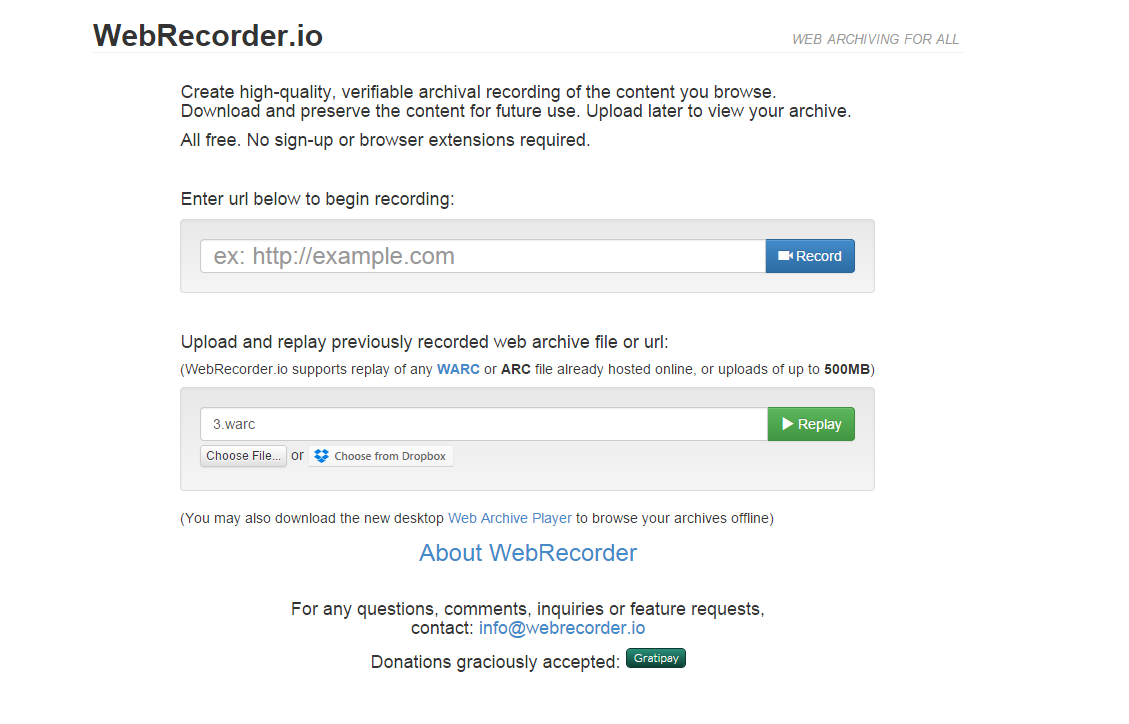
\includegraphics[scale=.7]{web1.png}
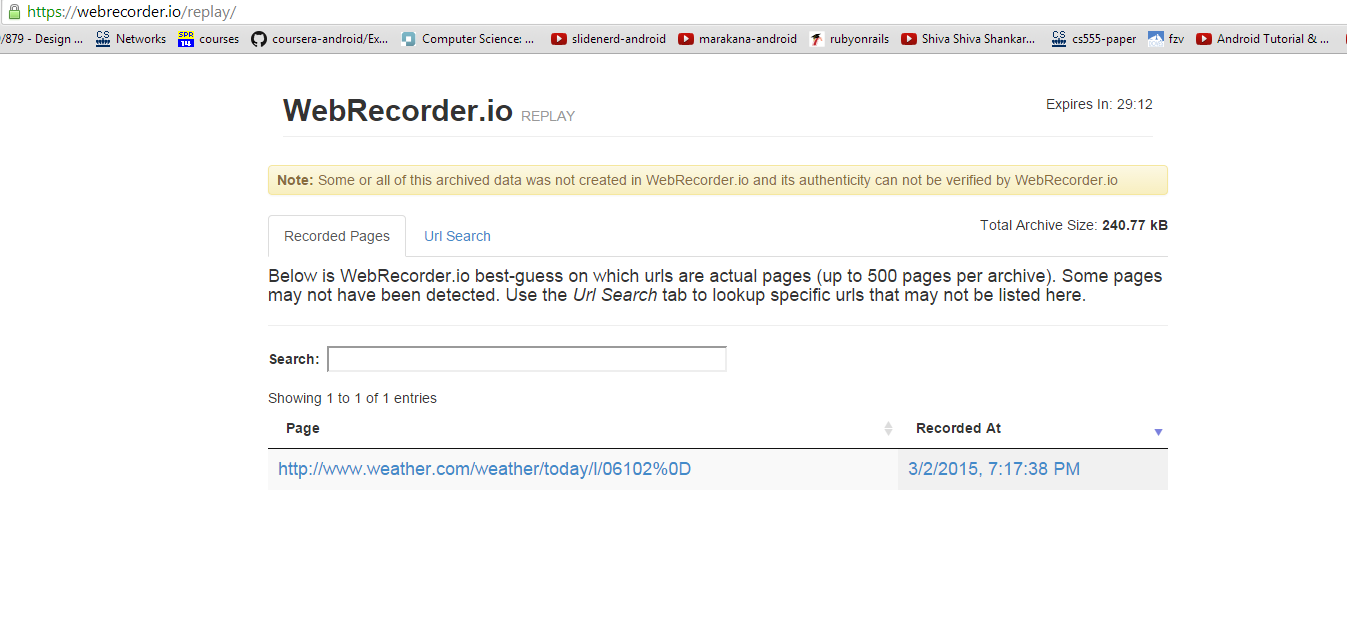
\includegraphics[scale=.5]{web2.png}
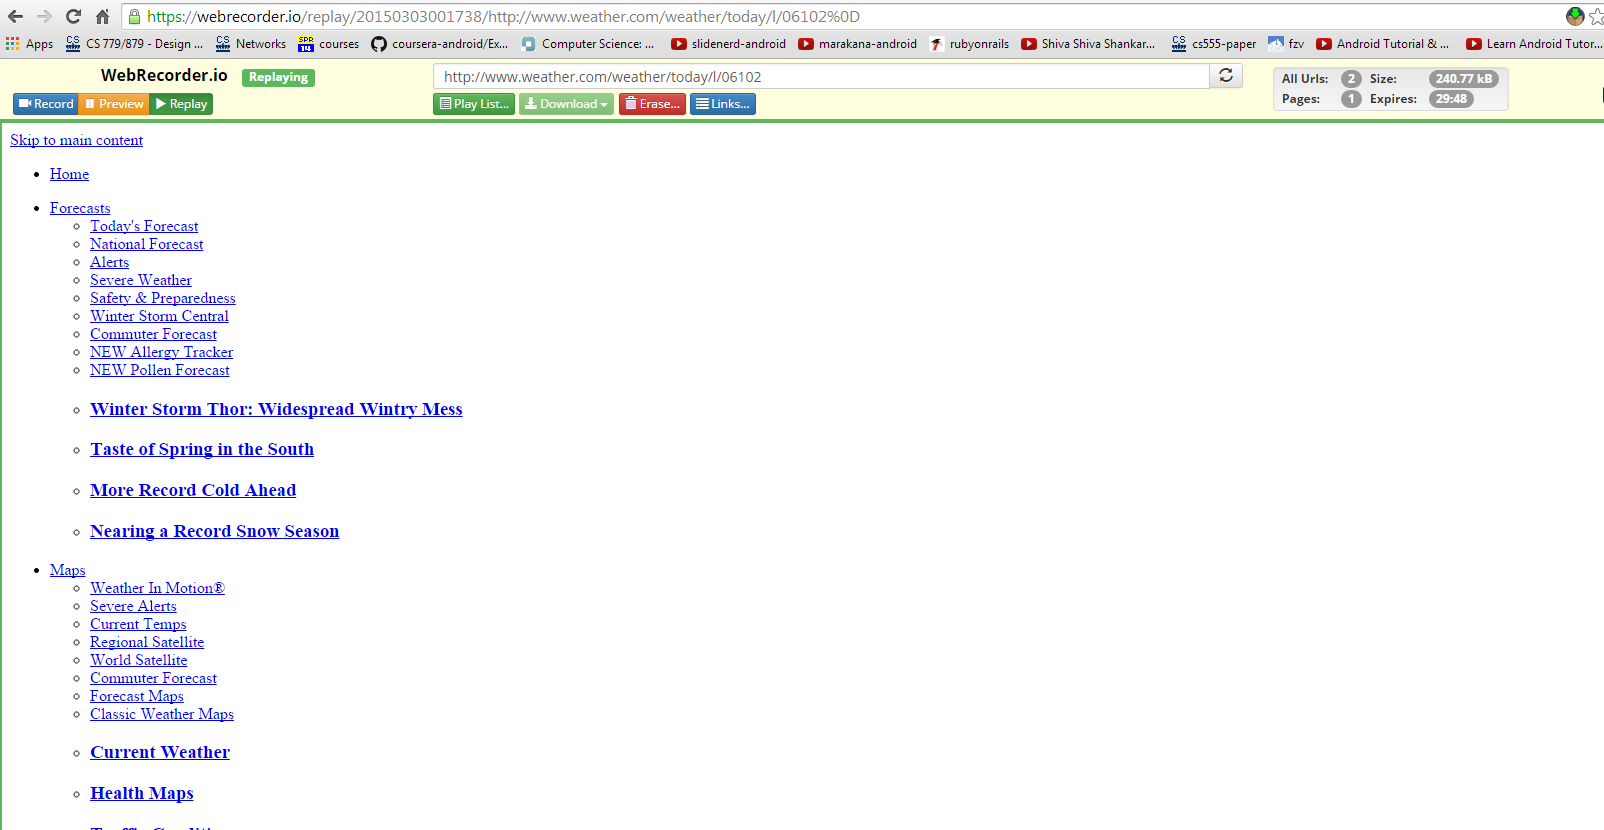
\includegraphics[scale=.4]{web3.png}
\end{center}

Playback using wayback machine via WAIL:
\begin{center}
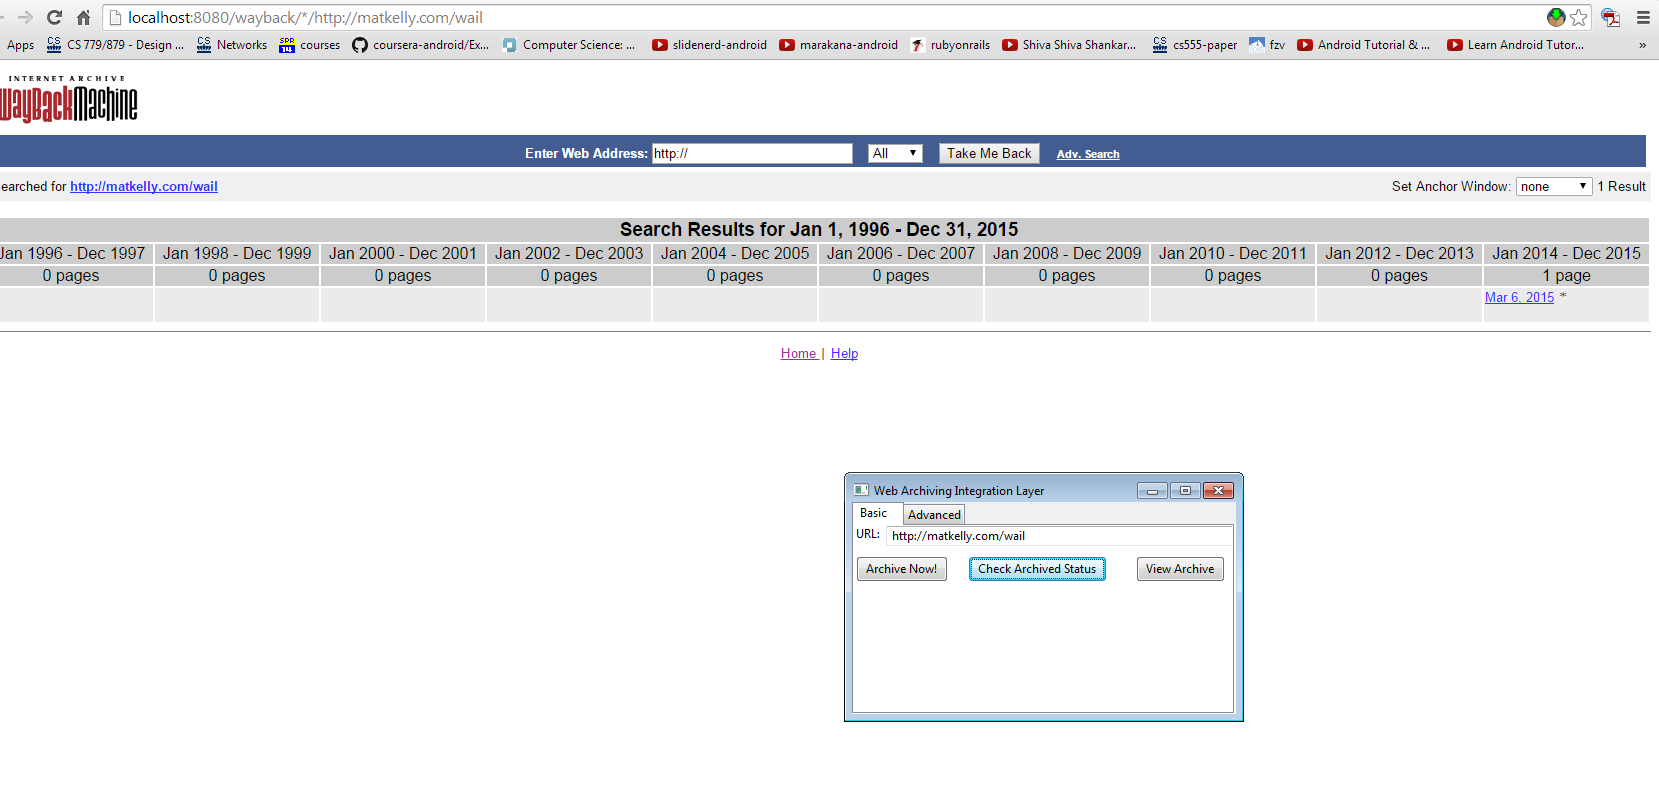
\includegraphics[scale=.4]{way1.png}
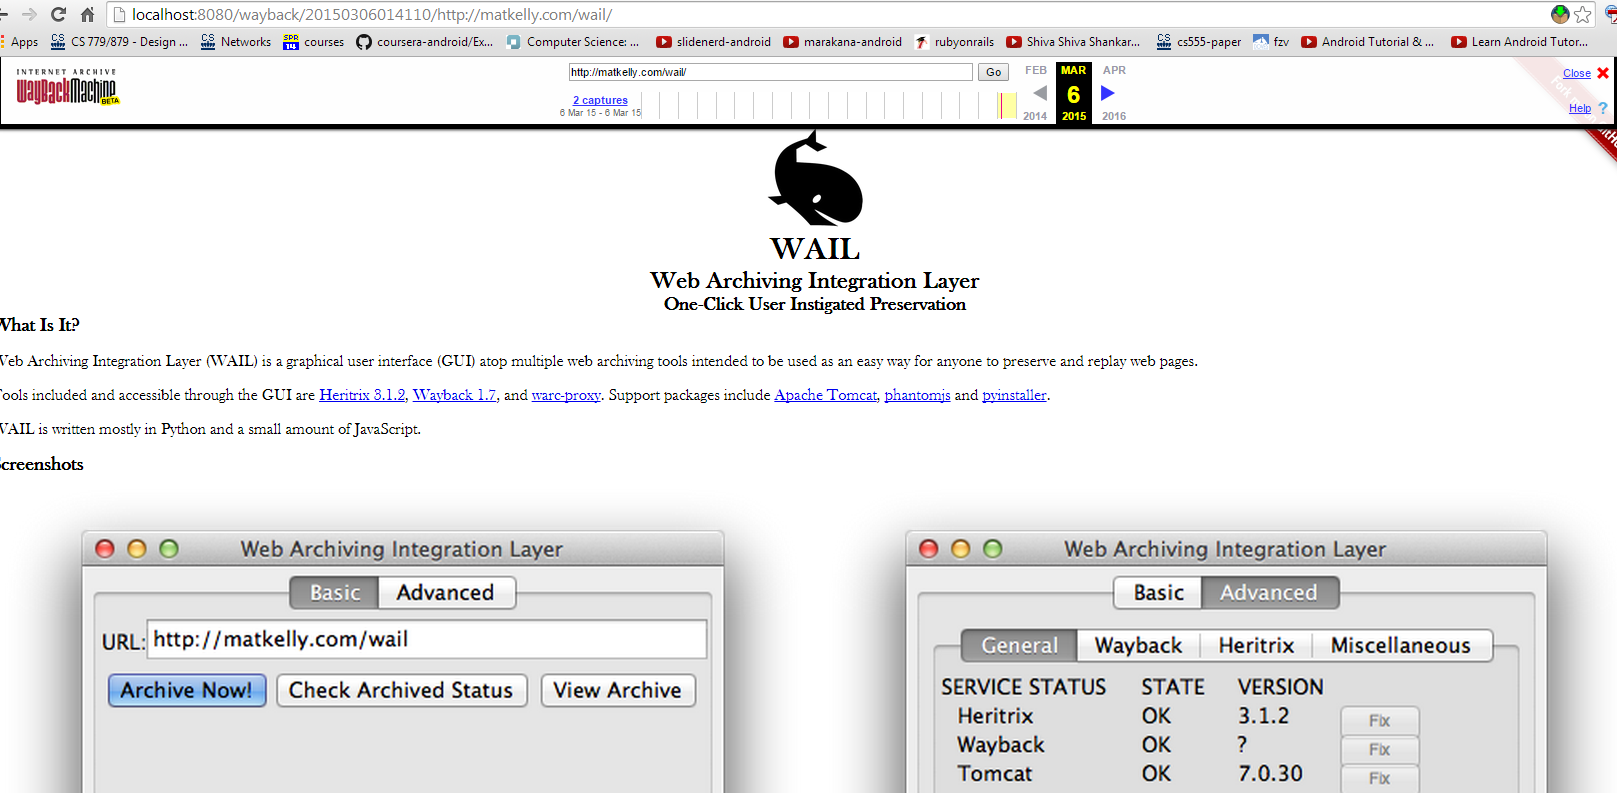
\includegraphics[scale=.4]{way2.png}
%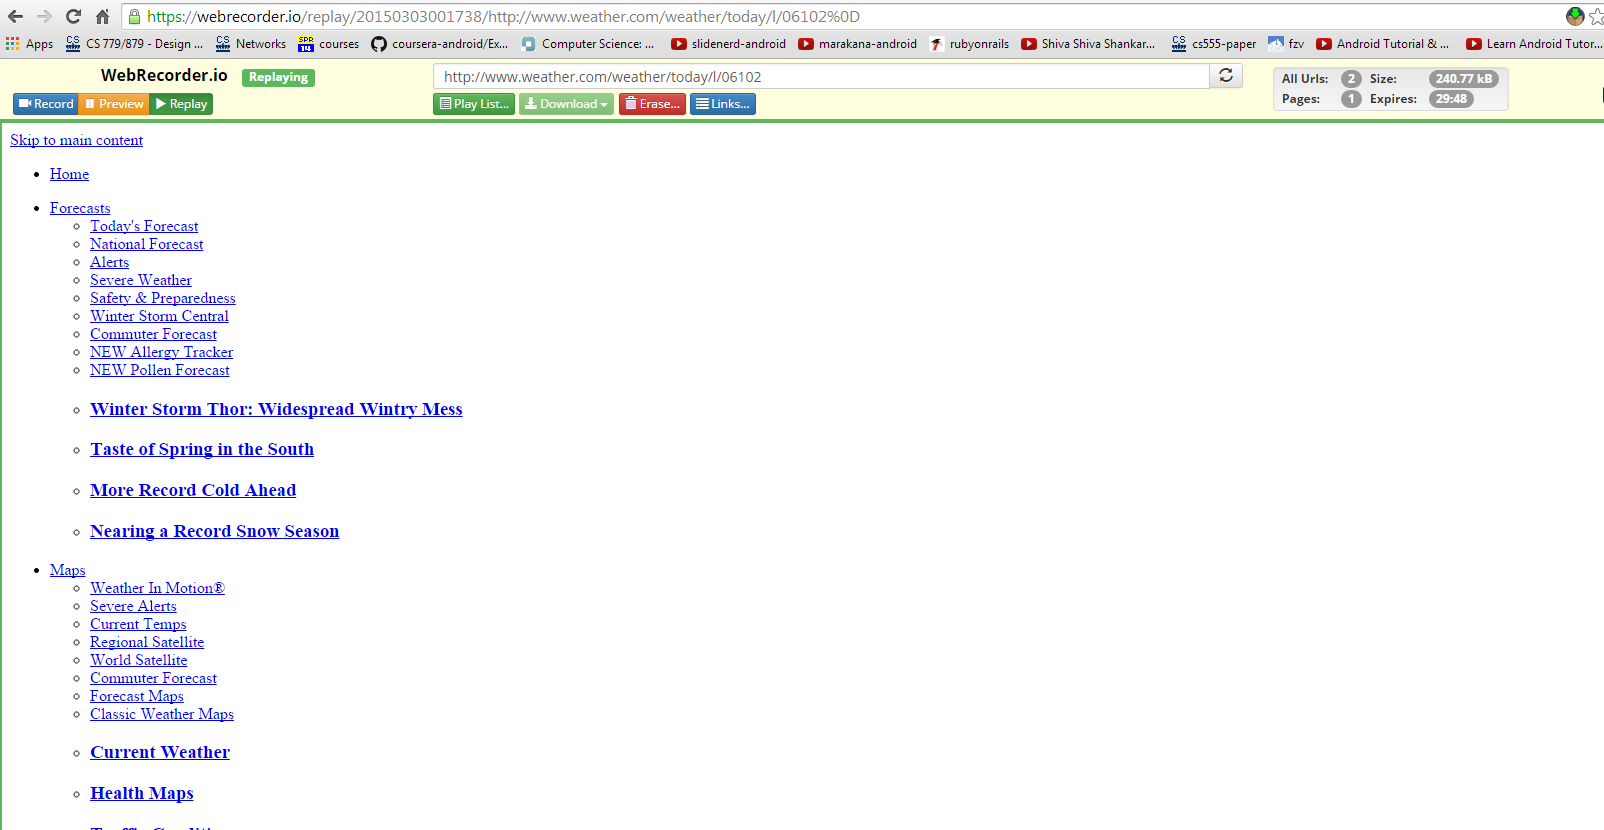
\includegraphics[scale=.5]{web3.png}
\end{center}








%------------------------------------------------

%\subsection{Heading on level 2 (subsection)}



%------------------------------------------------

%\subsubsection{Heading on level 3 (subsubsection)}

%\lipsum[3] % Dummy text

%\paragraph{Heading on level 4 (paragraph)}

%\lipsum[6] % Dummy text

%----------------------------------------------------------------------------------------
%	PROBLEM 2
%----------------------------------------------------------------------------------------

\section{Solr Instance}

To fire up a solr instance, in one terminal a solr server is started and in another terminal a java command is run along with location of .warc file this in turn will index the URL provided.The Solr UI is at http://localhost:8080/. To know if a given warc file has been indexed in the overview section of Solr view "statistics".
To query on an indexed URL the query section should be selected and a query should be written and execute query should be pressed to view the result.
Warcmerge is used to consolidate all the 100 warc files into one single warc file. All the dependencies for warcmerge are installed and warcmerge.py is run to consolidate all the 100 warc files. This single warc file is fed to solr and it gets indexed.
In the below diagram the value of the field wt is set to xml and the results are in xml format and also the value of the field rows is to set 10.
In the second Solar UI image the value of wt is set to json and the rows value to 1 and the results are in json format.
In the third image the value of facet is set to "true".

\begin{center}
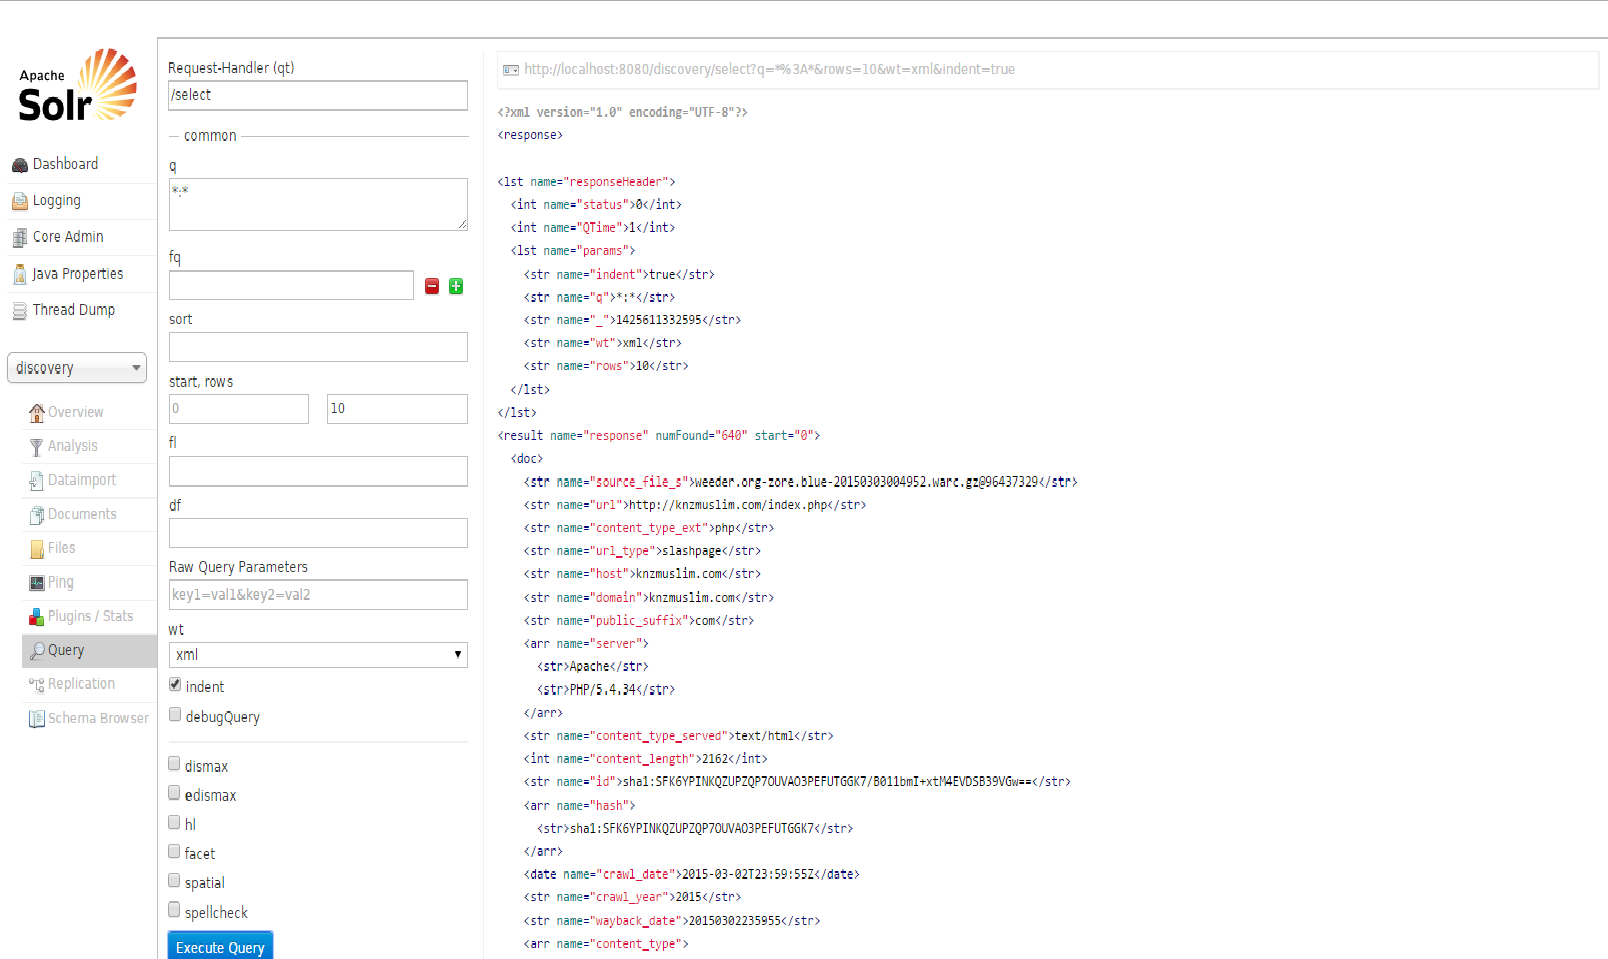
\includegraphics[scale=.4]{query1.png}
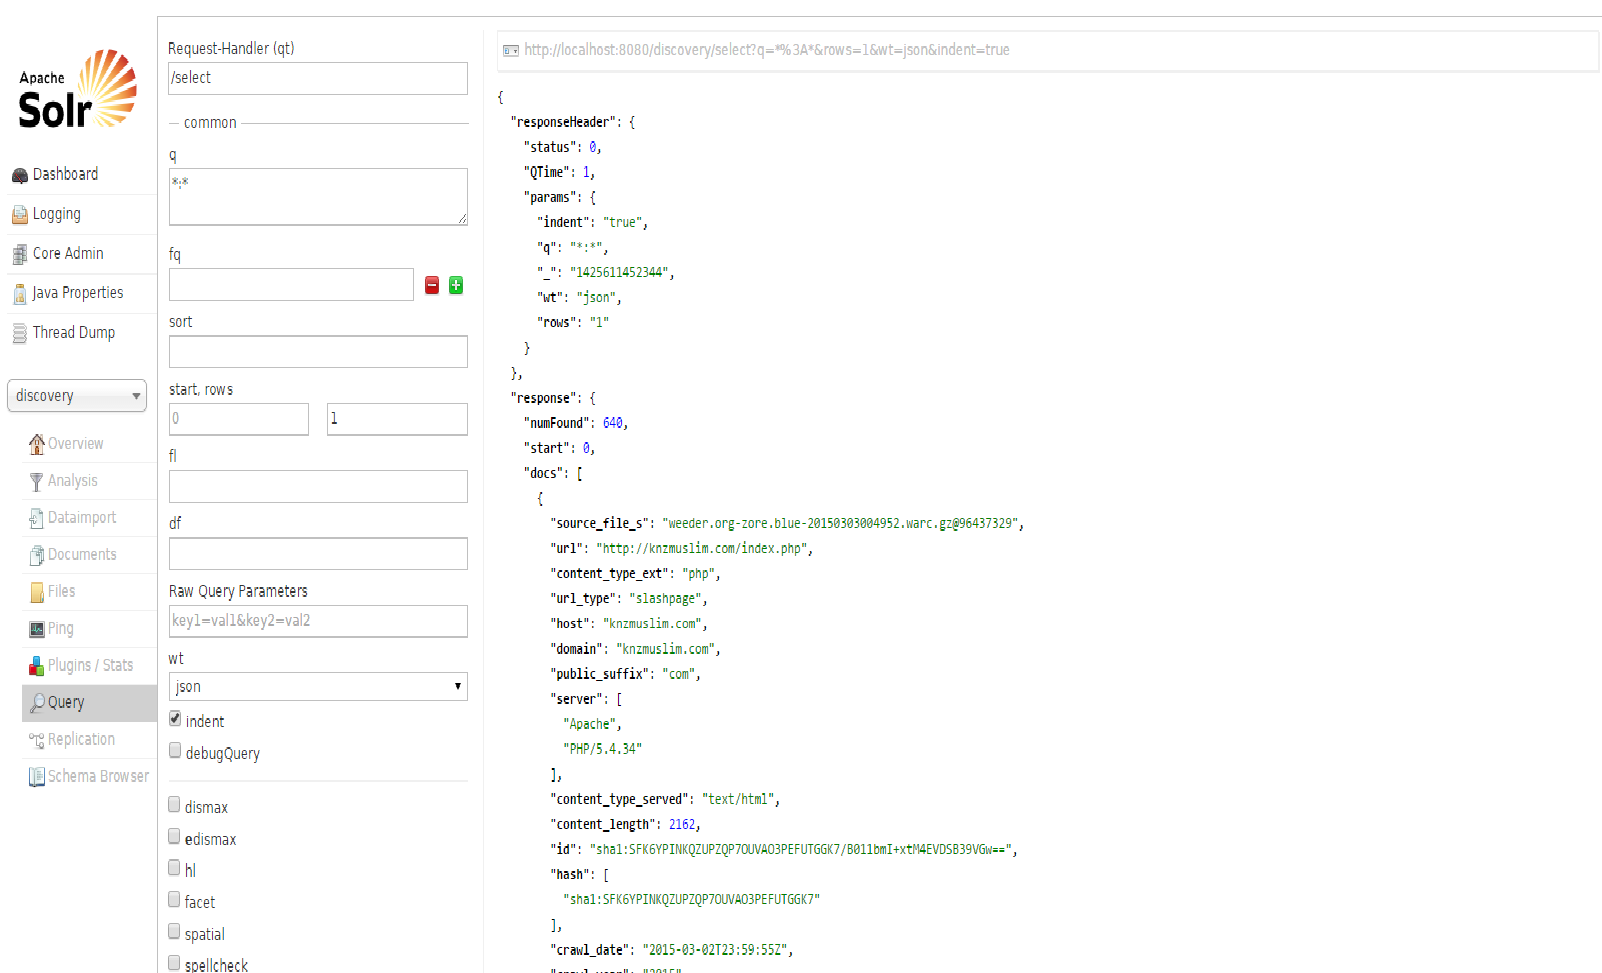
\includegraphics[scale=.4]{query2.png}
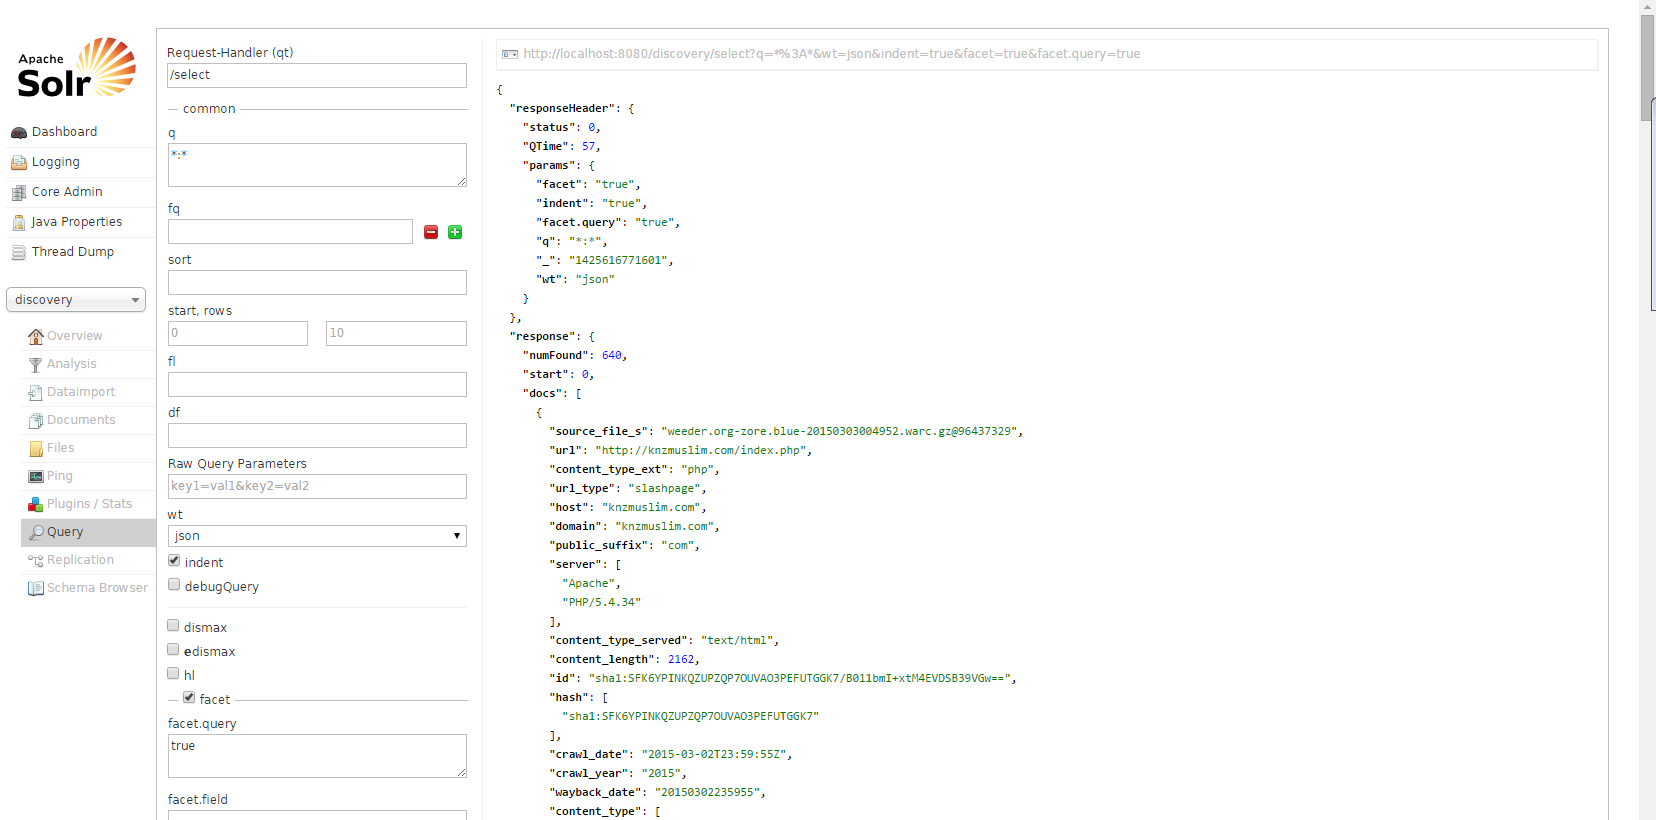
\includegraphics[scale=.4]{query3.png}
%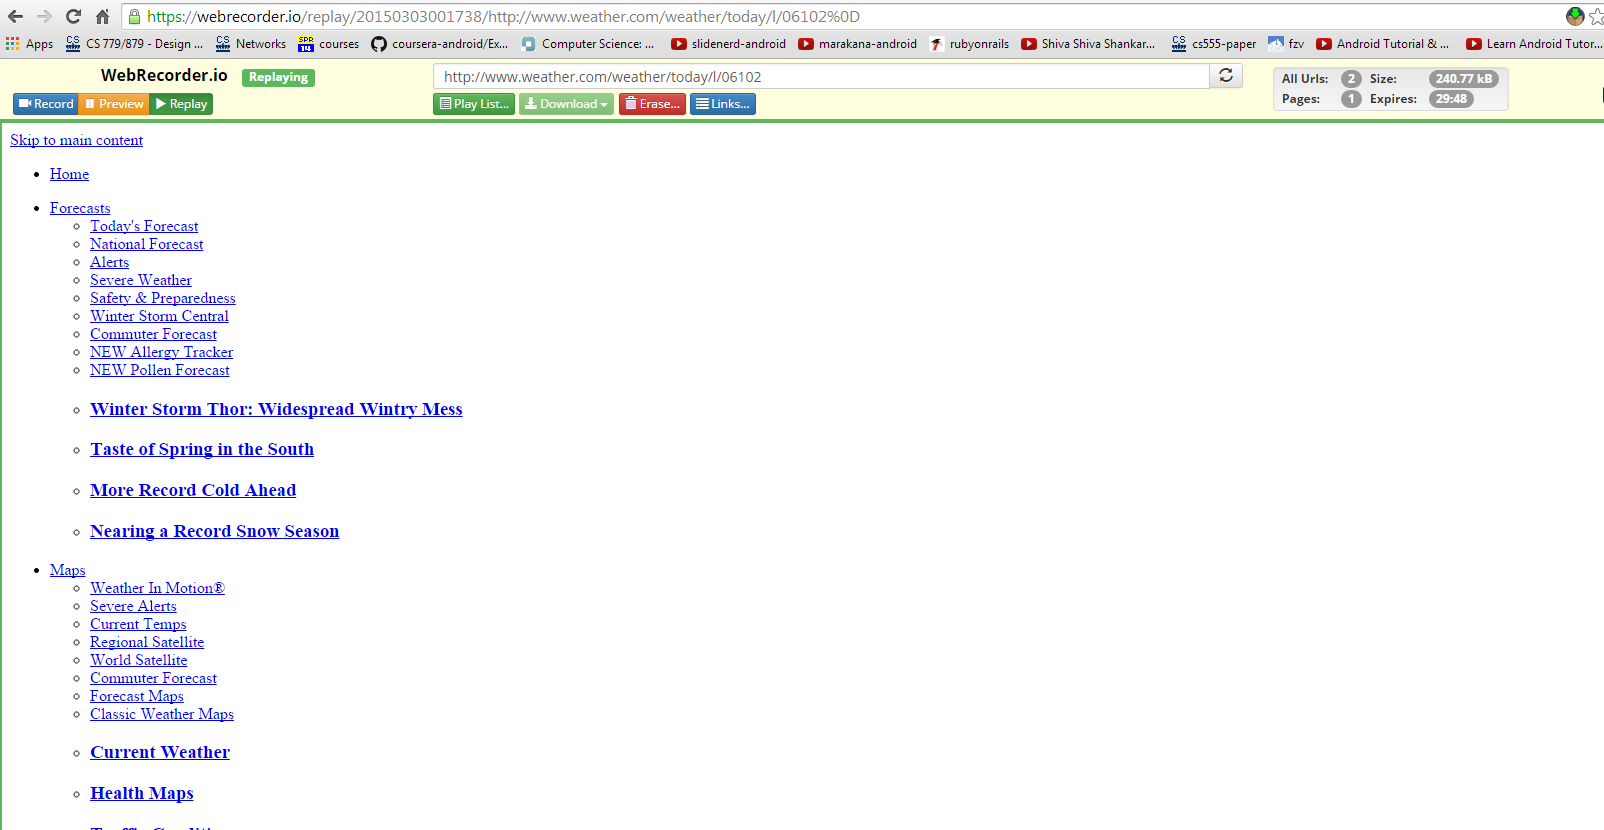
\includegraphics[scale=.5]{web3.png}
\end{center}



%------------------------------------------------


%------------------------------------------------



%----------------------------------------------------------------------------------------

\end{document}